% -*- mode: latex-mode; TeX-engine: xetex; LaTeX-command-style: (("" "SOURCE_DATE_EPOCH=0 %(PDF)%(latex) --shell-escape %S%(PDFout)")); TeX-master: "../dissertation.tex"; -*-

\chapter{Interaction of Single Atoms}
\label{ch:interaction-shift}

\section{Scattering Length}
\todo{}
(Importance/relation with binding energy etc.)

\section{Two Interacting Atoms in Optical Tweezer}

The Hamiltonian for two atoms in an harmonic potential with interaction is,
\[
  H=\sum_{i=x,y,z}\paren{\frac{m_{1}\omega_{1,i}^2r_{1,i}^2}{2}+\frac{p_{1,i}^2}{2m_{1}}}+\sum_{i=x,y,z}\paren{\frac{m_{2}\omega_{2,i}^2r_{2,i}^2}{2}+\frac{p_{2,i}^2}{2m_{2}}}+V_{int}\paren{\mathbf{r}_1-\mathbf{r}_2}\numberthis{eq:interaction-shift:orig-hamiltonian}
\]
where $m_j$ is the mass of the $j$-th atom,
$r_{j,i}$, $p_{j,i}$, $\omega_{j,i}$ are the coordinate, momentum and trapping frequency
for the $j$-th atom along the $i$-th axis.
$V_{int}$ is the interaction potential between the two atoms which is only a function
of the relative coordinate between the atoms $\mathbf{r}_1-\mathbf{r}_2$.

Since the two atoms experience the same trapping light field,
their trapping potential has the same center and the same shape.
However, due to the difference in the polarizability between the atoms,
the trap depth can be different.
Nevertheless, in our experiment, depending on the trapping wavelength,
we have $\omega_{1,i}\approx\omega_{2,i}$ to within $10\%$ to $20\%$
and this is the regime we will mainly focus on in this section.

The interaction potential $V_{int}$ is the original for
the molecular bound states and its exact form will be discussed in chapter \ref{ch:pa},
\ref{ch:raman-spectroscopy} and \ref{ch:raman-transfer}.
However, since the range of the potential is much smaller than
the size of the atomic wavefunction, we can ignore the short range details of the potential
and treat it as a contact interaction characterized only by the scattering length $a$.
\[
  V_{int}\paren{\mathbf{r}}=\frac{2\pi\hbar^2a}{\mu}\delta_{reg}\paren{\mathbf{r}}
\]
where $\mu = m_1m_2/\paren{m_1+m_2}$ is the reduced mass and
$\delta_{reg}\paren{\mathbf{r}}\equiv\delta^{(3)}\paren{\mathbf{r}}\paren{\partial/\partial r}r$
is the regularized delta-function.

In order to calculate the interaction term, we can change from the coordinates for
the two individual atoms to the center of mass (COM) and relative coordinates.
\begin{align*}
  R_i=&\ \frac{m_1r_{1,i}+m_2r_{2,i}}{m_1+m_2}&r_{rel,i}=&\ r_{1,i}-r_{2,i}\\
  P_i=&\ p_{1,i}+p_{2,i}&p_{rel,i}=&\ \frac{m_2p_{1,i}-m_1p_{2,i}}{m_1+m_2}
\end{align*}
The corresponding masses and trapping frequencies are,
\begin{align*}
  M=&\ m_1+m_2&\mu=&\ \frac{m_1m_2}{m_1+m_2}\\
  \Omega_i^2=&\ \frac{m_1\omega_{1,i}^2+m_2\omega_{2,i}^2}{m_1+m_2}&\omega_{rel,i}^2=&\ \frac{m_2\omega_{1,i}^2+m_1\omega_{2,i}^2}{m_1+m_2}
\end{align*}
and the Hamiltonian can be expressed as,
\begin{align*}
  \begin{split}
    H=&\sum_{i=x,y,z}\paren{\frac{M\Omega_{i}^2R_{i}^2}{2}+\frac{P_{i}^2}{2M}}+
    \left[\sum_{i=x,y,z}\paren{\frac{\mu\omega_{rel,i}^2r_{rel,i}^2}{2}+\frac{p_{rel,i}^2}{2\mu}}+
      V_{int}\paren{\mathbf{r}_{rel}}\right]\\
    &+\sum_{i=x,y,z}\mu\paren{\omega_{1,i}^2 - \omega_{2,i}^2}R_ir_{rel,i}
  \end{split}\numberthis{eq:interaction-shift:full-hamiltonian}
\end{align*}
The first term and the second term only relies on the COM motion and relative motion
respectively and can be solved independently. The third term mixes the COM and relative motion
and is proportional to the trapping frequency difference.
If the trapping frequencies are the same for the two atoms, the third term is $0$ and
the solution is fully separateable.
As mentioned above, since the trapping frequencies for the two atoms are similar,
we will assume the mixing term is small and treat it as a small correction in the calculation.

\subsection{Perturbative Calculation}
\label{ch:interaction-shift:theory:perturb}

For weak interaction, i.e. a small scattering length $a$, the effect of the interaction
on the energy level can be calculated perturbatively.
The result from this calculation is useful for checking the validity of the full calculation,
as well as providing an intuitive understanding of the shift and its dependency
on different parameters.

For simplicity, we will assume all the trapping frequencies are the same,
i.e. $\omega_{1,i}=\omega_{2,i}=\omega_{rel,i}=\Omega_i=\omega_i$,
so that we only need to consider the relative motion,
\[
  H_{rel}=\sum_{i=x,y,z}\paren{\frac{\mu\omega_{i}^2r_{rel,i}^2}{2}+\frac{p_{rel,i}^2}{2\mu}}+
  V_{int}\paren{\mathbf{r}_{rel}}
\]
When treating the interaction as perturbation, the base solution is the harmonic oscillator
states for the relative motion $|n_{rel,x},n_{rel,y},n_{rel,z}\rangle$.
The energy level pertubation is then,
\begin{align*}
  \Delta_{n_{rel,x},n_{rel,y},n_{rel,z}}=&\langle n_{rel,x},n_{rel,y},n_{rel,z}|V_{int}\paren{\mathbf{r}_{rel}}|n_{rel,x},n_{rel,y},n_{rel,z}\rangle\\
  =&\frac{2\pi\hbar^2a}{\mu}\langle n_{rel,x},n_{rel,y},n_{rel,z}|\delta_{reg}\paren{\mathbf{r}_{rel}}|n_{rel,x},n_{rel,y},n_{rel,z}\rangle\\
  =&\frac{2\pi\hbar^2a}{\mu}\abs{\psi_{n_{rel,x},n_{rel,y},n_{rel,z}}(0)}^2\numberthis{eq:interaction-shift-perturb-shift}
\end{align*}
where $\abs{\psi_{n_{rel,x},n_{rel,y},n_{rel,z}}(0)}^2$ is the probability density
for zero distance between the atoms.

For the motional ground state, the shift is,
\begin{align*}
  \Delta_{0,0,0}=&a\frac{2\hbar^2}{\mu\sqrt{\pi}}\prod_{i=x,y,z}\frac{1}{\beta_{rel,i}}
\end{align*}
where $\beta_{rel,i}\equiv\sqrt{\hbar/\mu\omega_{rel,i}}$ is the relative motion
oscillator length along the $i$-th axis.
The shift is proportional to the strength of the interaction $a$,
and is also stronger for stronger confinement where the wavefunction density is higher.

We can see from (\ref{eq:interaction-shift-perturb-shift}) that the shift is only
non-zero when all of $n_{rel,i}$'s are even.
The shift is also smaller for higher motional excited state with smaller wavefunction density.
This means that the shift will only be observable if the atom is cooled to closed to
the motional ground state and will be small or zero for hot atoms.

\subsection{Non-perturbative Calculation}

The first order perturbative result breaks down for large $a$ when the energy shift
approaches the motional energy scale $\omega_{rel,i}$.
Moreover, due to the divergence nature of the delta-function in the contact interaction potential,
higher order perturbative calculation does not converge.
It is therefore necessary to use a non-perturbative solution of the interacting atoms
in order to interprete measurement of the shift for strong interaction.
To do this, we first ignore the last term in the Hamiltonian
\ref{eq:interaction-shift:full-hamiltonian} so that it is fully separable
into COM and relative motion.

For the relative Hamiltonian, we use the analytic cylindrical solutions
from Ref.~\cite{idziaszek_analytical_2006}.
These solutions require the potential to be cylindrically symmetric and
that the ratio between the radial trapping frequency
and the axial trapping frequency $\eta\equiv\omega_{radial}/\omega_{axial}$
to be an integer.
We therefore define $\eta = 6$, which is close to the actual values of $5.6$
and ignores the $7 \%$ difference between the two radial trapping frequencies
in order to use these solutions.
These differences from the real Hamiltonian will be included later,
together with the mixing term, as a correction.
The analytic solutions are only given for the interacting states,
but there also many relative states which have zero wavefunction at the $\delta$-function,
and therefore are unaffected.
We have identified these states from the perturbative calculation
in section \ref{ch:interaction-shift:theory:perturb}
which are states with $l\ne0$ or odd $m_z$
after transforming to the cylindrical coordinate used by the analytic solution,
where $l$ is the angular momentum quantum numbers for the radial part,
and $m_z$ is quantum number for 1D harmonic oscillator for the axial part.
The complete basis includes both the interacting states from
Ref.~\cite{idziaszek_analytical_2006} as well as all of the non-interacting states.
The non-interacting states are solutions to the cylindrical harmonic oscillator,
and so are just cylindrical harmonic oscillator wavefunctions with eigenenergies
\begin{align*}
  \frac{E_{n,l,m_z}}{\hbar\omega_z}=&\paren{2 n + |l| + 1}\eta + \paren{m_z + 1/2}
                                      \numberthis{eq:interaction-shift:cylind-E}
\end{align*}
where $n$ is the principle quantum number for the radial part.
In order to find the non-interacting wavefunction,
we need to remove the interaction wavefunction from
the cylindrical harmonic oscillator wavefunctions.
The complication in this process is that when $\eta$ is an integer,
as is required by the solution of the interaction,
there is a subspace of cylindrical harmonic oscillator states with $l=0$
and even $m_z$ that are degenerate from Eq.~\ref{eq:interaction-shift:cylind-E}.
In each degenerate subspace with $N_{\mathrm{deg}}$ states,
the non-interacting states $\psi_{non-int}$
are a linear superposition of the degenerate eigenstates $\psi_i$
that satisfies the condition $V_{int}\psi_{non-int} = 0$ or
$\psi_{non-int}\paren{\mathbf{r}_{rel}=0}=0$.
We find these amplitudes $c_i$ using a Gram-Schmidt procedure,
which from the requirement $\sum_{i=1}^{N_{\mathrm{deg}}}  c_i \psi_i\paren{\mathbf{r}_{rel}=0} = 0$.
In each subspace, there is only one interacting state,
for which the analytic solution is used, and  $N_{\mathrm{deg}}-1$ non-interacting states.

For the interacting states,
the energies are given by the transcendental equations~\cite{idziaszek_analytical_2006}
\begin{align*}
  \mathcal{F}\paren{-\frac{\paren{E-E_0}}{2} , \eta}=&-\frac{\sqrt{2\pi}}{a}
\end{align*}
where $\mathcal{F}\paren{x, \eta}$ is given by
\begin{align*}
  \mathcal{F}\paren{x, \eta}=
  &\frac{\sqrt{\pi} \Gamma(x)}{\Gamma(x+\frac{1}{2})}
    \sum_{m=1}^{n-1} F\paren{1,x;x+\frac{1}{2} ; e^{i(2\pi m/ \eta )}}
    -\frac{2 \sqrt{\pi} \Gamma(x)}{\Gamma(x-\frac{1}{2})}
\end{align*}
Here $F(a,b;c,x)$ denotes the hypergeometric function
and $\Gamma(x)$ is the Euler gamma function.
The energy $E$ and $E_0$ are in units of the axial trap energy $\hbar \omega_z$,
and so the ground state energy $E_0  = \eta + 1/2$.

The COM Hamiltonian is a cylindrical harmonic oscillator and the energies is given by
Eq.~\ref{eq:interaction-shift:cylind-E}.

\begin{figure}
  \centering
  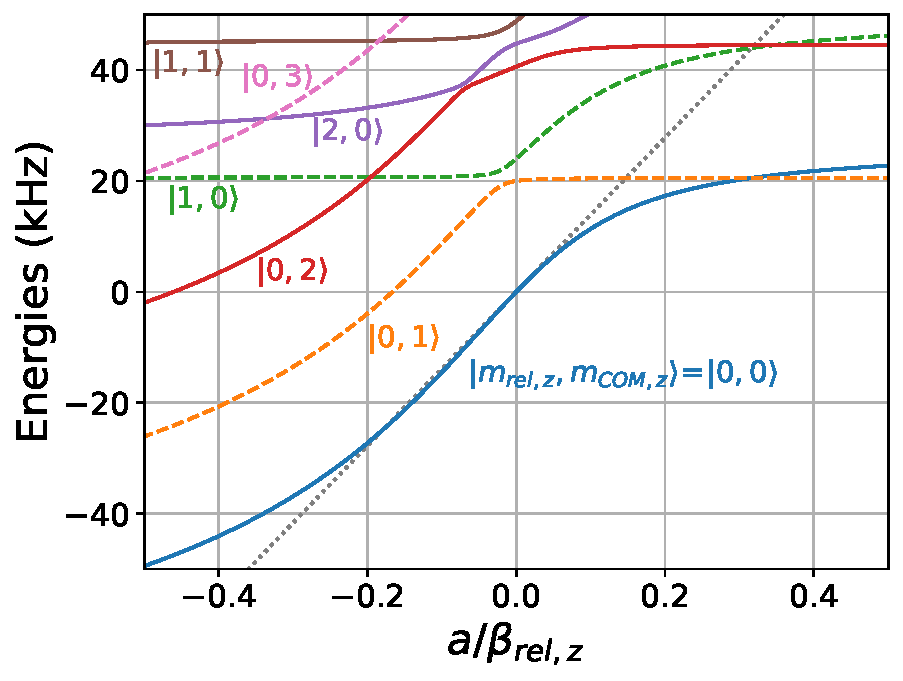
\includegraphics[width=0.7\textwidth]{figures/interaction_shift_energies.pdf}
  \caption[Result of interaction shift calculation.]{
    Energy levels as a function of scattering length
    (in unit of the axial relative motion oscillator length
    $\beta_{rel,z}$) from the non-perturbative calculation.
    The dashed straight light is the result from first order perturbation
    for the motional ground state which shows good agreement with the exact calculation
    at small scattering length.
    Only states that are in the radial motional (both relative and COM) ground state
    are shown because of the high radial motional energy scale ($100\mathrm{kHz}$).
    The states are labeled with their relative and COM axial motional quantum numbers
    $m_{rel,z}$ and $m_{COM,z}$.
    Due to the relative and COM motion mixing term and the resulting avoided crossings
    in the energy levels, these are not true quantum number
    and are not constants along the same line.
    The number shown in the plot are for the state at large negative scattering length.
    States with even total parity, i.e. $m_{rel,z} + m_{COM,z}$, are plotted in solid lines
    whereas ones with odd total parity are plotted in dashed lines.
    Since the Hamiltonian conserves total parity,
    there is no coupling between the between the two sets of states
    which results in the level crossing shown in the plot.
    \label{fig:interaction-shift:energies}}
\end{figure}

Now that we have the solution in the separable and cylindrical case,
the next step is to include the non-separable and asymmetric correction terms
by diagonalizing the total matrix in the combined COM and relative cylindrical bases.
Compared to treating the interaction term in \ref{eq:interaction-shift:orig-hamiltonian}
as a perturbation, the correction terms included here all have the form of
harmonic potentials and therefore have much better convergence behavior.
We include all states with energies up to $20 \omega_{rel,z}$ in the calculation.
The matrix elements are calculated numerically using the cylindrical wavefunctions,
which for completeness are given here:
\begin{align*}
  \Psi_{n,l,m_z}\paren{\rho,\theta,z}=
  &\Psi^{\mathrm{radial}}_{n,l}\paren{\rho, \theta}\Psi^{\mathrm{axial}}_{m_z}\paren{z}
\end{align*}
with the normalized radial harmonic oscillator wavefunction,
\begin{align*}
  \Psi^{\mathrm{radial}}_{n,l}\paren{\rho, \theta}=
  &\sqrt{\frac{2n!}{a_\perp^2 (n+|l|)!}} e^{-r^2/(2 a_\perp^2)} \paren{\frac{r}{a_\perp}}^{|l|}
    L_n^{|l|}\paren{\frac{r^2}{a_\perp^2}} \frac{ e^{i l \theta}}{\sqrt{2 \pi}}
\end{align*}
and the normalized 1D harmonic wavefunction,
\begin{align*}
  \Psi^{\mathrm{axial}}_{m_z}(z)=&\frac{1}{\sqrt{2^{m_z} m_z!}} \frac{1}{\sqrt{a_z}(\pi)^{1/4}}
                                   e^{-z^2/(2 a_z)} H_{m_z}( z/a_z)
\end{align*}
Here the radial and axial oscillator lengths are defined as
$a_\perp = \sqrt{\hbar/( \mu \omega_\perp)}$ and $a_z = \sqrt{\hbar/ (\mu \omega_z)}$.
$H_{m_z}$ are the Hermite-Gaussian functions,
and $L^{|l|}_n$ are the generalized Laguerre polynomials.

The eigenenergies of the matrix are calculated as a function of the scattering length.
The results for the lowest energy ones are shown in Fig.~\ref{fig:interaction-shift:energies}.

\section{Interaction Shift Spectroscopy}

\subsection{Experiment Sequence}
The absolute energies shown in Fig.~\ref{fig:interaction-shift:energies} have an arbitrary global
offset and are therefore not directly measurable.
Instead, the measurable quantities are the energy differences between different states,
which can be done either by changing the scattering length, i.e. moving along the x axis,
or by changing the motional state of the atoms, i.e. moving along the y axis.

In our experiment, we measure the interaction shifts by flipping the spin state of
one but not the other atom using Raman transition.
Since the scattering length depends on the spin state,
this allow us to measure the difference between energy levels for different scattering lengths
by comparing the resonance frequency in the absence of the other atom \todo{figure}.
The spin flip is done in the same $8.8 \mathrm{G}$ we use for Raman sideband cooling
(section \ref{ch:rsc:setup}).
We drive the transition using two Raman beams that are co-propagating
which imprints no phase gradient on the atomic wavefunction (section \ref{ch:rsc-basic-theory-raman}).
This reduces the number of observable resonances and provides a cleaner spectrum since,
\begin{enumerate}
\item Parity is conserved during the transition.\\
  Starting from the motional ground state, this means that all dashed lines in
  Fig.~\ref{fig:interaction-shift:energies} are uncoupled.
\item Coupling to different motional states are surpressed.\\
  In particular, this reduces the coupling to COM motional states in the strong
  interaction limit and to motional states for the unaddressed atom in the weak interaction limit.
\end{enumerate}

\subsection{Results}
\label{ch:interaction-shift:result}
(motional sideband, scattering length result)

\section{Summary and Outlook}
(Motional state selection)
